\chapter{Arhitektura i dizajn sustava}
		
		Pri razvoju web aplikacije Zamjena soba koristi se stil višeslojne arhitekture (engl. multi-layer architecture). To znači da uključuje više logičkih slojeva implementacije programske potpore. Općenito, osnova svih višeslojnih stilova je troslojni stil arhitekture koji sadrži:
		\begin{itemize}
		\item 	korisnički ili prezentacijski sloj (engl. presentation layer) – sloj s korisničkim sučeljem, odnosno onaj koji korisnik vidi i koji mu služi za unos podataka; uneseni podaci se mogu pohraniti u bazu ili u datotečni sustav
		\item 	sloj poslovne logike (engl. logic layer) – sloj s implementacijom poslovnih procesa i izračuna; pomoću njega se odvija sva komunikacija s bazom; on obrađuje i generira dinamički sadržaj 
		\item 	podatkovni sloj (engl. data layer) – sloj za pohranu podataka u bazu ili u datotečni sustav.
		\end{itemize}
		
		No,  klijentsku i poslužiteljsku stranu moguće je organizirati u više slojeva, pri čemu svaki sloj pruža uslugu nekom drugom.
	U slučaju naše aplikacije, u kojoj koristimo radni okvir Spring Boot, bilo je potrebno dodati više slojeva, te su slojevi arhitekture naše aplikacije:
		\begin{itemize}
		\item 	sloj korisničke strane – implementiran u JavaScriptu, koristi knjižnicu React koja omogućuje prikaz korisničkog sučelja. Pisan je u radnoj okolini Microsoft Visual Studio Code.
		\item 	sloj nadglednika (engl. controller) – povezuje korisničku stranu s poslužiteljskom stranom.
		\item 	sloj usluge (engl. service) – obavlja svu poslovnu logiku i potrebne izračune.
		\item 	sloj domene (engl. domain) – ima razrađeni model podataka domene
		\item 	sloj za pristup podatcima (engl. data access object, DAO) – omogućuje spremanje i dohvat podataka iz baze podataka te razmjenu tih podataka sa slojem domene
		\item 	sloj baze podataka – omogućuje pohranu podataka u relacijsku bazu PostgreSQL
	\end{itemize}
		
		
		Svi slojevi osim prvog i zadnjeg, pisani su na radnoj platformi Eclipse u programskom jeziku Java.
		\newline
		\hspace* {8mm} Primijetimo da slojevi naglednika, usluge i domene su analogni MVC arhitekturi. Odnosno sloj domene (domain) predstavlja model, sloj usluge (service) predstavlja view, te sloj naglednika (controller) predstavlja controller.
		\newline
		\hspace* {8mm} Izabrali smo baš tu arhitekturu kako bismo mogli bolje podijeliti rad među članovima tima (princip podijeli pa vladaj).
		\newline
		\hspace* {8mm} Nakon stavljanja aplikacije na server pomoću platforme Heroku, web poslužitelj je taj koji isporučuje sadržaj web aplikacije. To izvršava preko HTTP protokola na portu 8080.
		\newline
		\hspace* {8mm} Komunikacija među slojevima izvršava se u pozadini putem određenih portova (vrata). Sloj korisničke strane povezan je sa slojem nadglednika preko aplikacijskog programskog sučelja (API) na portu 3000. Sloj nadglednika, usluge i domene te sloj za pristup podacima su zajedno integrirani, odnosno povezuje ih radni okvir Spring Boot. Naposlijetku, sloj za pristup podacima je povezan sa slojem baze podataka preko porta 5432.
		
		
		

				
		\section{Baza podataka}
			
			
		\hspace{10mm} Koristi se relacijska baza podataka, ona se sastoji od skupa povezanih tablica odnosno relacija. Izabrali smo DBMS (database management system) PostgreSQL.
		\newline
		Entiteti baze su:
		\begin{itemize}
		\item \textit{student}
		\item \textit{sc}
		\item \textit{dom}
		\item \textit{menza}
		\item \textit{soba}
		\item \textit{filter}
		\item \textit{grad}
		\item \textit{oglas}
		\item \textit{lajkani\textunderscore oglas}
		\item \textit{moguca\textunderscore zamjena}
		\item \textit{zakljucane\textunderscore zamjene}
		\end{itemize}
		
			\subsection{Opis tablica}
			

				\hspace{10mm} \textbf{Student}
				\newline
				- u ovoj tablici se nalazi popis svih studenata i djelatnika studentskih centara.
				\newline
				\textit{Primarni ključ: id}
				
				
				\begin{longtabu} to \textwidth {|X[8, l]|X[6, l]|X[20, l]|}
					
					\hline \multicolumn{3}{|c|}{\textbf{student}}	 \\[3pt] \hline
					\endfirsthead
					
					\hline \multicolumn{3}{|c|}{\textbf{student}}	 \\[3pt] \hline
					\endhead
					
					\hline 
					\endlastfoot
					
					\cellcolor{LightGreen} id & BIGINT	&  	svakom korisniku se automatski generira id (identifikacijski broj)	\\ \hline
					username	& VARCHAR &  korisnik ga sam odabire, jedinstven je 	\\ \hline 
					email & VARCHAR & email korisnika, jedinstven je  \\ \hline 
					JMBAG & VARCHAR	& JMBAG korisnika		\\ \hline 
					name & VARCHAR	&  ime i prezime korisnika		\\ \hline 
					user\textunderscore role & INT	& sustav dodijeljuje ovlasti kako bi razlikovao studente od SC djelatnika		\\ \hline 
					password & VARCHAR	&  hash lozinke		\\ \hline 
					locked & BOOLEN	&  osposobljenost ili neosposobljenost korisnikovog računa		\\ \hline 
					enabled & BOOLEAN	&  aktiviranost ili deaktiviranost korisnikovog računa		\\ \hline 
					potvrdjeni\textunderscore lanac & BIGINT	&  id lanca u kojem je potvrđen, dog ga nema vrijednost mu je null		\\ \hline 
					
					
				\end{longtabu}
				
				
				\textbf{Studentski centar}
				\newline
				\textit{Primarni ključ: idSC}
				\newline
				\textit{Strani ključ: grad\textunderscore id\textunderscore grada}
				\newline
				
				
				\begin{longtabu} to \textwidth {|X[6, l]|X[6, l]|X[20, l]|}
					
					\hline \multicolumn{3}{|c|}{\textbf{SC}}	 \\[3pt] \hline
					\endfirsthead
					
					\hline \multicolumn{3}{|c|}{\textbf{SC}}	 \\[3pt] \hline
					\endhead
					
					\hline 
					\endlastfoot
					
					\cellcolor{LightGreen}idSC & BGIINT	&  	svakom studentskom centru se automatski dodjeljuje id	\\ \hline
					ime	& VARCHAR & naziv studentskog centra  	\\ \hline 
					grad\textunderscore id\textunderscore grada & INT & grad u kojem se nalazi studentski centar  \\ \hline 
					
					
					
				\end{longtabu}
				
				
				
				
				\textbf{Dom}
				\newline
				\textit{Primarni ključ: id\textunderscore dom}
				\newline
				\textit{Strani ključ: menza\textunderscore naziv\textunderscore menze, sc\textunderscore idsc, grad\textunderscore id\textunderscore grada}
				\newline
			
				
				\begin{longtabu} to \textwidth {|X[14, l]|X[6, l]|X[20, l]|}
					
					\hline \multicolumn{3}{|c|}{\textbf{dom}}	 \\[3pt] \hline
					\endfirsthead
					
					\hline \multicolumn{3}{|c|}{\textbf{dom}}	 \\[3pt] \hline
					\endhead
					
					\hline 
					\endlastfoot
					
					\cellcolor{LightGreen}id\textunderscore dom & BIGINT	&  	svakom studentskom domu se automatski dodjeljuje id	\\ \hline
					ime<c doma	& VARCHAR & naziv doma  	\\ \hline 
					grad\textunderscore id\textunderscore grada & INT & grad u kojem se dom nalazi  \\ \hline 
					najbliza\textunderscore menza\textunderscore naziv\textunderscore menze & VARCHAR	&  naziv najblize menze		\\ \hline 
					\cellcolor{LightBlue}sc\textunderscore idSC	& BIGINT &  id studentskog centra u kojem se nalazi 	\\ \hline 
					
					
				\end{longtabu}
				
				
				\textbf{Menza}
				\newline
				- najbliža menza studentskom domu
				\newline
				\textit{Primarni ključ: naziv\textunderscore menze}
				\newline
				\textit{Strani ključ: grad\textunderscore id\textunderscore grada}
				
				
				
				\begin{longtabu} to \textwidth {|X[6, l]|X[6, l]|X[20, l]|}
					
					\hline \multicolumn{3}{|c|}{\textbf{menza}}	 \\[3pt] \hline
					\endfirsthead
					
					\hline \multicolumn{3}{|c|}{\textbf{menza}}	 \\[3pt] \hline
					\endhead
					
					
					\cellcolor{LightGreen}naziv\textunderscore menze & VARCHAR	&  	naziv menze	\\ \hline
					grad\textunderscore id\textunderscore grada	& INT & id grada u kojem se nalazi  	\\ \hline 
					
					
					
				\end{longtabu}
				
				
				\textbf{Soba}
				\newline
				- studentova sobe
				\newline
				\textit{Primarni ključ: id\textunderscore soba}
				\newline
				\textit{Strani ključ: id\textunderscore doma\textunderscore id\textunderscore dom, id\textunderscore studenta\textunderscore id}
				
				
				
				\begin{longtabu} to \textwidth {|X[8, l]|X[6, l]|X[20, l]|}
					
					\hline \multicolumn{3}{|c|}{\textbf{soba}}	 \\[3pt] \hline
					\endfirsthead
					
					\hline \multicolumn{3}{|c|}{\textbf{soba}}	 \\[3pt] \hline
					\endhead
					
					\hline 
					\endlastfoot
					
					\cellcolor{LightGreen}id\textunderscore soba & BIGINT	&  	svakoj sobi se automatski dodjeljuje jedinstveni id	\\ \hline
					kat	& SMALLINT & kat na kojem se nalazi  	\\ \hline 
					kategorija\textunderscore sobe	& SMALLINT & kategorija sobe studentskog doma (od 1 do 7)  	\\ \hline 
					paviljon	& SMALLINT & paviljon u kojem se nalazi  	\\ \hline
					id\textunderscore doma\textunderscore id\textunderscore dom	& BIGINT & id doma u kojem se nalazi  	\\ \hline
					id\textunderscore studenta\textunderscore id	& BIGINT & id studenta koji raspolaže tom sobom  	\\ \hline 
					
					
					
				\end{longtabu}
				
				
				\textbf{Filter}
				\newline
				- služi za filtriranje oglasa na početnoj stranici
				\newline
				\textit{Primarni ključ: id\textunderscore filter}
				\newline
				\textit{Strani ključ: id\textunderscore doma\textunderscore id\textunderscore dom, id\textunderscore studenta\textunderscore id}
				
				
				
				\begin{longtabu} to \textwidth {|X[8, l]|X[6, l]|X[20, l]|}
					
					\hline \multicolumn{3}{|c|}{\textbf{filter}}	 \\[3pt] \hline
					\endfirsthead
					
					\hline \multicolumn{3}{|c|}{\textbf{filter}}	 \\[3pt] \hline
					\endhead
					
					\hline 
					\endlastfoot
					
					\cellcolor{LightGreen}id\textunderscore filter & BIGINT	&  	svakome filteru se automatski dodjeljuje jedinstveni id	\\ \hline
					kat	& SMALLINT & kat koji se pretražuje  	\\ \hline 
					kategorija\textunderscore sobe	& SMALLINT & kategorija sobe koja se pretražuje  	\\ \hline 
					paviljon	& SMALLINT & paviljon koji se pretražuje  	\\ \hline
					id\textunderscore doma\textunderscore id\textunderscore dom	& BIGINT & id doma koji se pretražuje  	\\ \hline
					student\textunderscore id	& BIGINT & id studenta koji koji je napravio filter  	\\ \hline 
					
					
					
				\end{longtabu}
				
				
				\textbf{Grad}
				\newline
				\textit{Primarni ključ: id\textunderscore grada}
				
				
				
				\begin{longtabu} to \textwidth {|X[6, l]|X[6, l]|X[20, l]|}
					
					\hline \multicolumn{3}{|c|}{\textbf{grad}}	 \\[3pt] \hline
					\endfirsthead
					
					\hline \multicolumn{3}{|c|}{\textbf{grad}}	 \\[3pt] \hline
					\endhead
					
					\hline 
					\endlastfoot
					
					\cellcolor{LightGreen}id\textunderscore grada & INT	&  	svakome gradu se automatski dodjeljuje jedinstveni id	\\ \hline
					ime\textunderscore grada	& VARCHAR & naziv grada  	\\ \hline 
					
					
					
				\end{longtabu}
				
				
				\textbf{Oglas}
				\newline
				- oglas kojime student nudi svoju sobu
				\newline
				\textit{Primarni ključ: id\textunderscore oglas}
				\newline
				\textit{Strani ključ: dom\textunderscore id\textunderscore dom, student\textunderscore id}
				
				
				\begin{longtabu} to \textwidth {|X[7, l]|X[6, l]|X[20, l]|}
					
					\hline \multicolumn{3}{|c|}{\textbf{oglas}}	 \\[3pt] \hline
					\endfirsthead
					
					\hline \multicolumn{3}{|c|}{\textbf{oglas}}	 \\[3pt] \hline
					\endhead
					
					\hline 
					\endlastfoot
					
					\cellcolor{LightGreen}id\textunderscore oglas & BIGINT	&  	svakome oglasu se automatski dodjeljuje jedinstveni id	\\ \hline
					aktivan	& BOOLEAN & student može deaktivirati aktivan oglas  	\\ \hline 
					kat	& SMALLINT & kat na kojem se nalazi studentova soba  	\\ \hline 
					kategorija\textunderscore sobe	& SMALLINT & kategorija studentove sobe  	\\ \hline 
					paviljon	& SMALLINT & paviljon u kojem se nalazi studentova soba  	\\ \hline
					dom\textunderscore id\textunderscore dom	& BIGINT & id doma u kojem se nalazi studentova soba  	\\ \hline
					student\textunderscore id	& BIGINT & id studenta koji je sastavio oglas  	\\ \hline 
					
					
					
				\end{longtabu}
				
				
				\textbf{Lajkani oglas}
				\newline
				- lajkovi koji povezuju studenta i oglas koji je on lajkao
				\newline
				\textit{Primarni ključ: oglas\textunderscore id, student\textunderscore id}
				
				
				\begin{longtabu} to \textwidth {|X[7, l]|X[6, l]|X[20, l]|}
					
					\hline \multicolumn{3}{|c|}{\textbf{lajkani\textunderscore oglas}}	 \\[3pt] \hline
					\endfirsthead
					
					\hline \multicolumn{3}{|c|}{\textbf{lajkani\textunderscore oglas}}	 \\[3pt] \hline
					\endhead
					
					\hline 
					\endlastfoot
					
					\cellcolor{LightGreen}oglas\textunderscore id & BIGINT	&  	id lajkanog oglasa	\\ \hline
					\cellcolor{LightBlue}student\textunderscore id & BIGINT	&  	id studenta koji je lajkao oglas	\\ \hline
					stupanj\textunderscore lajkanja	& INT & Može biti: 1, 2 ili 3 ovisno o pritisutom broju srca. Također može biti 0 za uklananje lajka te 4 za opciju "ne prikazuj više"  	\\ \hline 
					procitano	& BOOLEAN & Služi za obavještavanje autora oglasa o novim dobivenim lajkovima  	\\ \hline 
					
					
				\end{longtabu}
				
				
				\textbf{Moguća zamjena}
				\newline
				- služi za prikaz ostvarivih zamjena korisniku
				\newline
				\textit{Primarni ključ: id\textunderscore lanca, redni\textunderscore broj}
				\newline
				\textit{Strani ključ: oglas\textunderscore id\textunderscore oglas}
				
				
				\begin{longtabu} to \textwidth {|X[6, l]|X[6, l]|X[20, l]|}
					
					\hline \multicolumn{3}{|c|}{\textbf{moguca\textunderscore zamjena}}	 \\[3pt] \hline
					\endfirsthead
					
					\hline \multicolumn{3}{|c|}{\textbf{moguca\textunderscore zamjena}}	 \\[3pt] \hline
					\endhead
					
					\hline 
					\endlastfoot
					
					\cellcolor{LightGreen}id\textunderscore lanca & BIGINT	&  	svakome lancu zamjena se automatski dodjeljuje jedinstveni id	\\ \hline
					\cellcolor{LightBlue}redni\textunderscore broj & SMALLINT	&  	Redni broj oglasa u lancu zamjena 	\\ \hline
					oglas\textunderscore id\textunderscore oglas	& BIGINT & id oglasa studentovog oglasa u lancu zamjena	\\ \hline 
					procitano	& BOOLEAN & Služi za obavještavanje autora oglasa o novim mogućim zamjenama  	\\ \hline 
					
					
				\end{longtabu}
				
				
				
				\textbf{Zaključane zamjene}
				\newline
				- potvrđene zamjene soba od strane studenata, koje se prikazuju djelatnku studentskog centra
				\newline
				\textit{Primarni ključ: id\textunderscore zamjene}
				\newline
				\textit{Strani ključ: oglas1\textunderscore id\textunderscore oglas, oglas2\textunderscore id\textunderscore oglas}
				
				
				\begin{longtabu} to \textwidth {|X[7, l]|X[6, l]|X[20, l]|}
					
					\hline \multicolumn{3}{|c|}{\textbf{zakljucane\textunderscore zamjene}}	 \\[3pt] \hline
					\endfirsthead
					
					\hline \multicolumn{3}{|c|}{\textbf{zakljucane\textunderscore zamjene}}	 \\[3pt] \hline
					\endhead
					
					
					\hline 
					\endlastfoot
					
					id\textunderscore zamjene & BIGINT	&  	svakoj zaključanoj zamjeni se automatski dodjeljuje jedinstveni id	\\ \hline
					aktivan & BOOLEAN	&  	izvršenost zamjene	\\ \hline
					oglas1\textunderscore id\textunderscore oglas	& BIGINT & id oglasa 1 u zamjeni  	\\ \hline 
					oglas2\textunderscore id\textunderscore oglas	& BIGINT & id oglasa 2 u zamjeni  	\\ \hline
					
				\end{longtabu}
				
				\eject
				
				
			
			\subsection{Dijagram baze podataka}
			Priložen je ER-model (entity realtionship model) baze podataka. Strani ključevi su prikazani crtom među tablicama. Plava točka označava da u toj tablici se nalazi strani ključ koji je u povezanoj tablici primarni ključ.
			\newline
			
			\begin{figure}[H]
			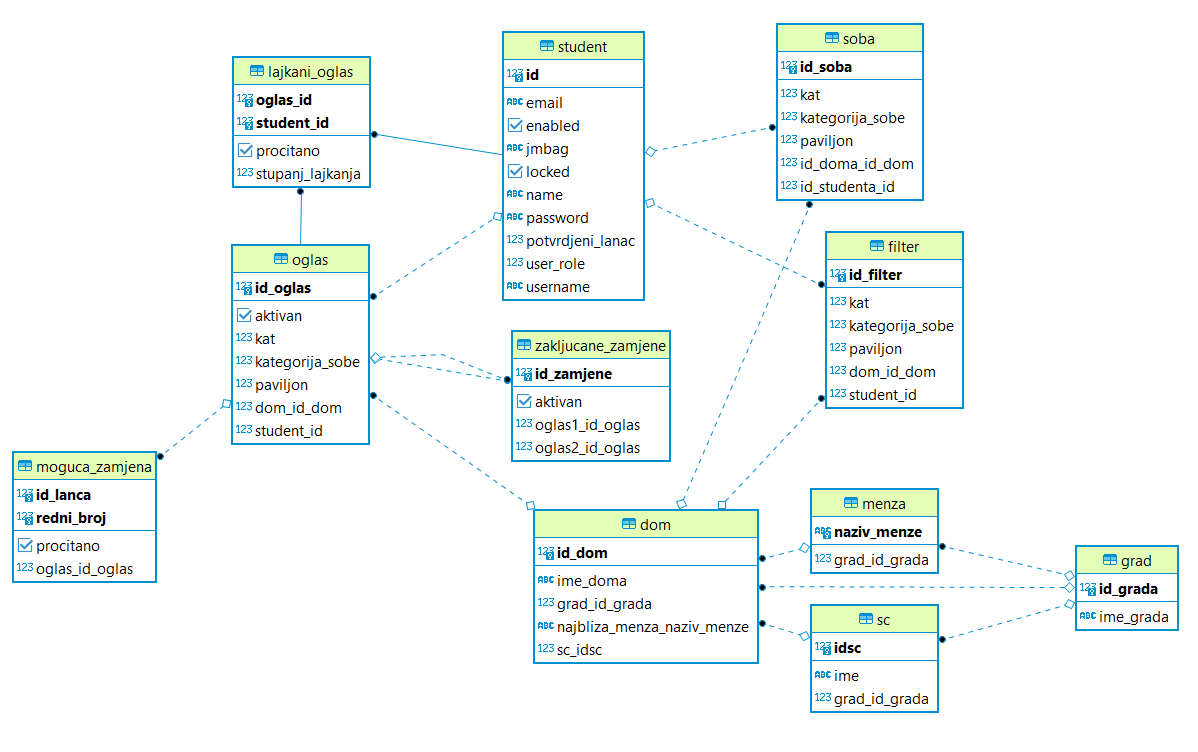
\includegraphics[scale=0.7]{slike/novi_er_model.png} 
			\centering
			\caption{Dijagram baze podataka}
			\label{fig:baza}
		\end{figure}
		
\eject
			
			
			
		\section{Dijagram razreda}
		
		Na slici 4.1 je prikazan potupuni dijagram razreda. Stavke su grupirane prema odgovarajućem paketu unutar kojeg se nalaze. Zbog lakšeg prikaza, kružićima su označena sučelja.
		\newline
		JWT (JSON Web Token) služi za identifikaciju korisnika. On dodjeljuje token svakom korisniku. Preko toga se svi korisnikovi zahtjevi mogu ispuniti u web aplikaciji.
		
		\begin{figure}[H]
			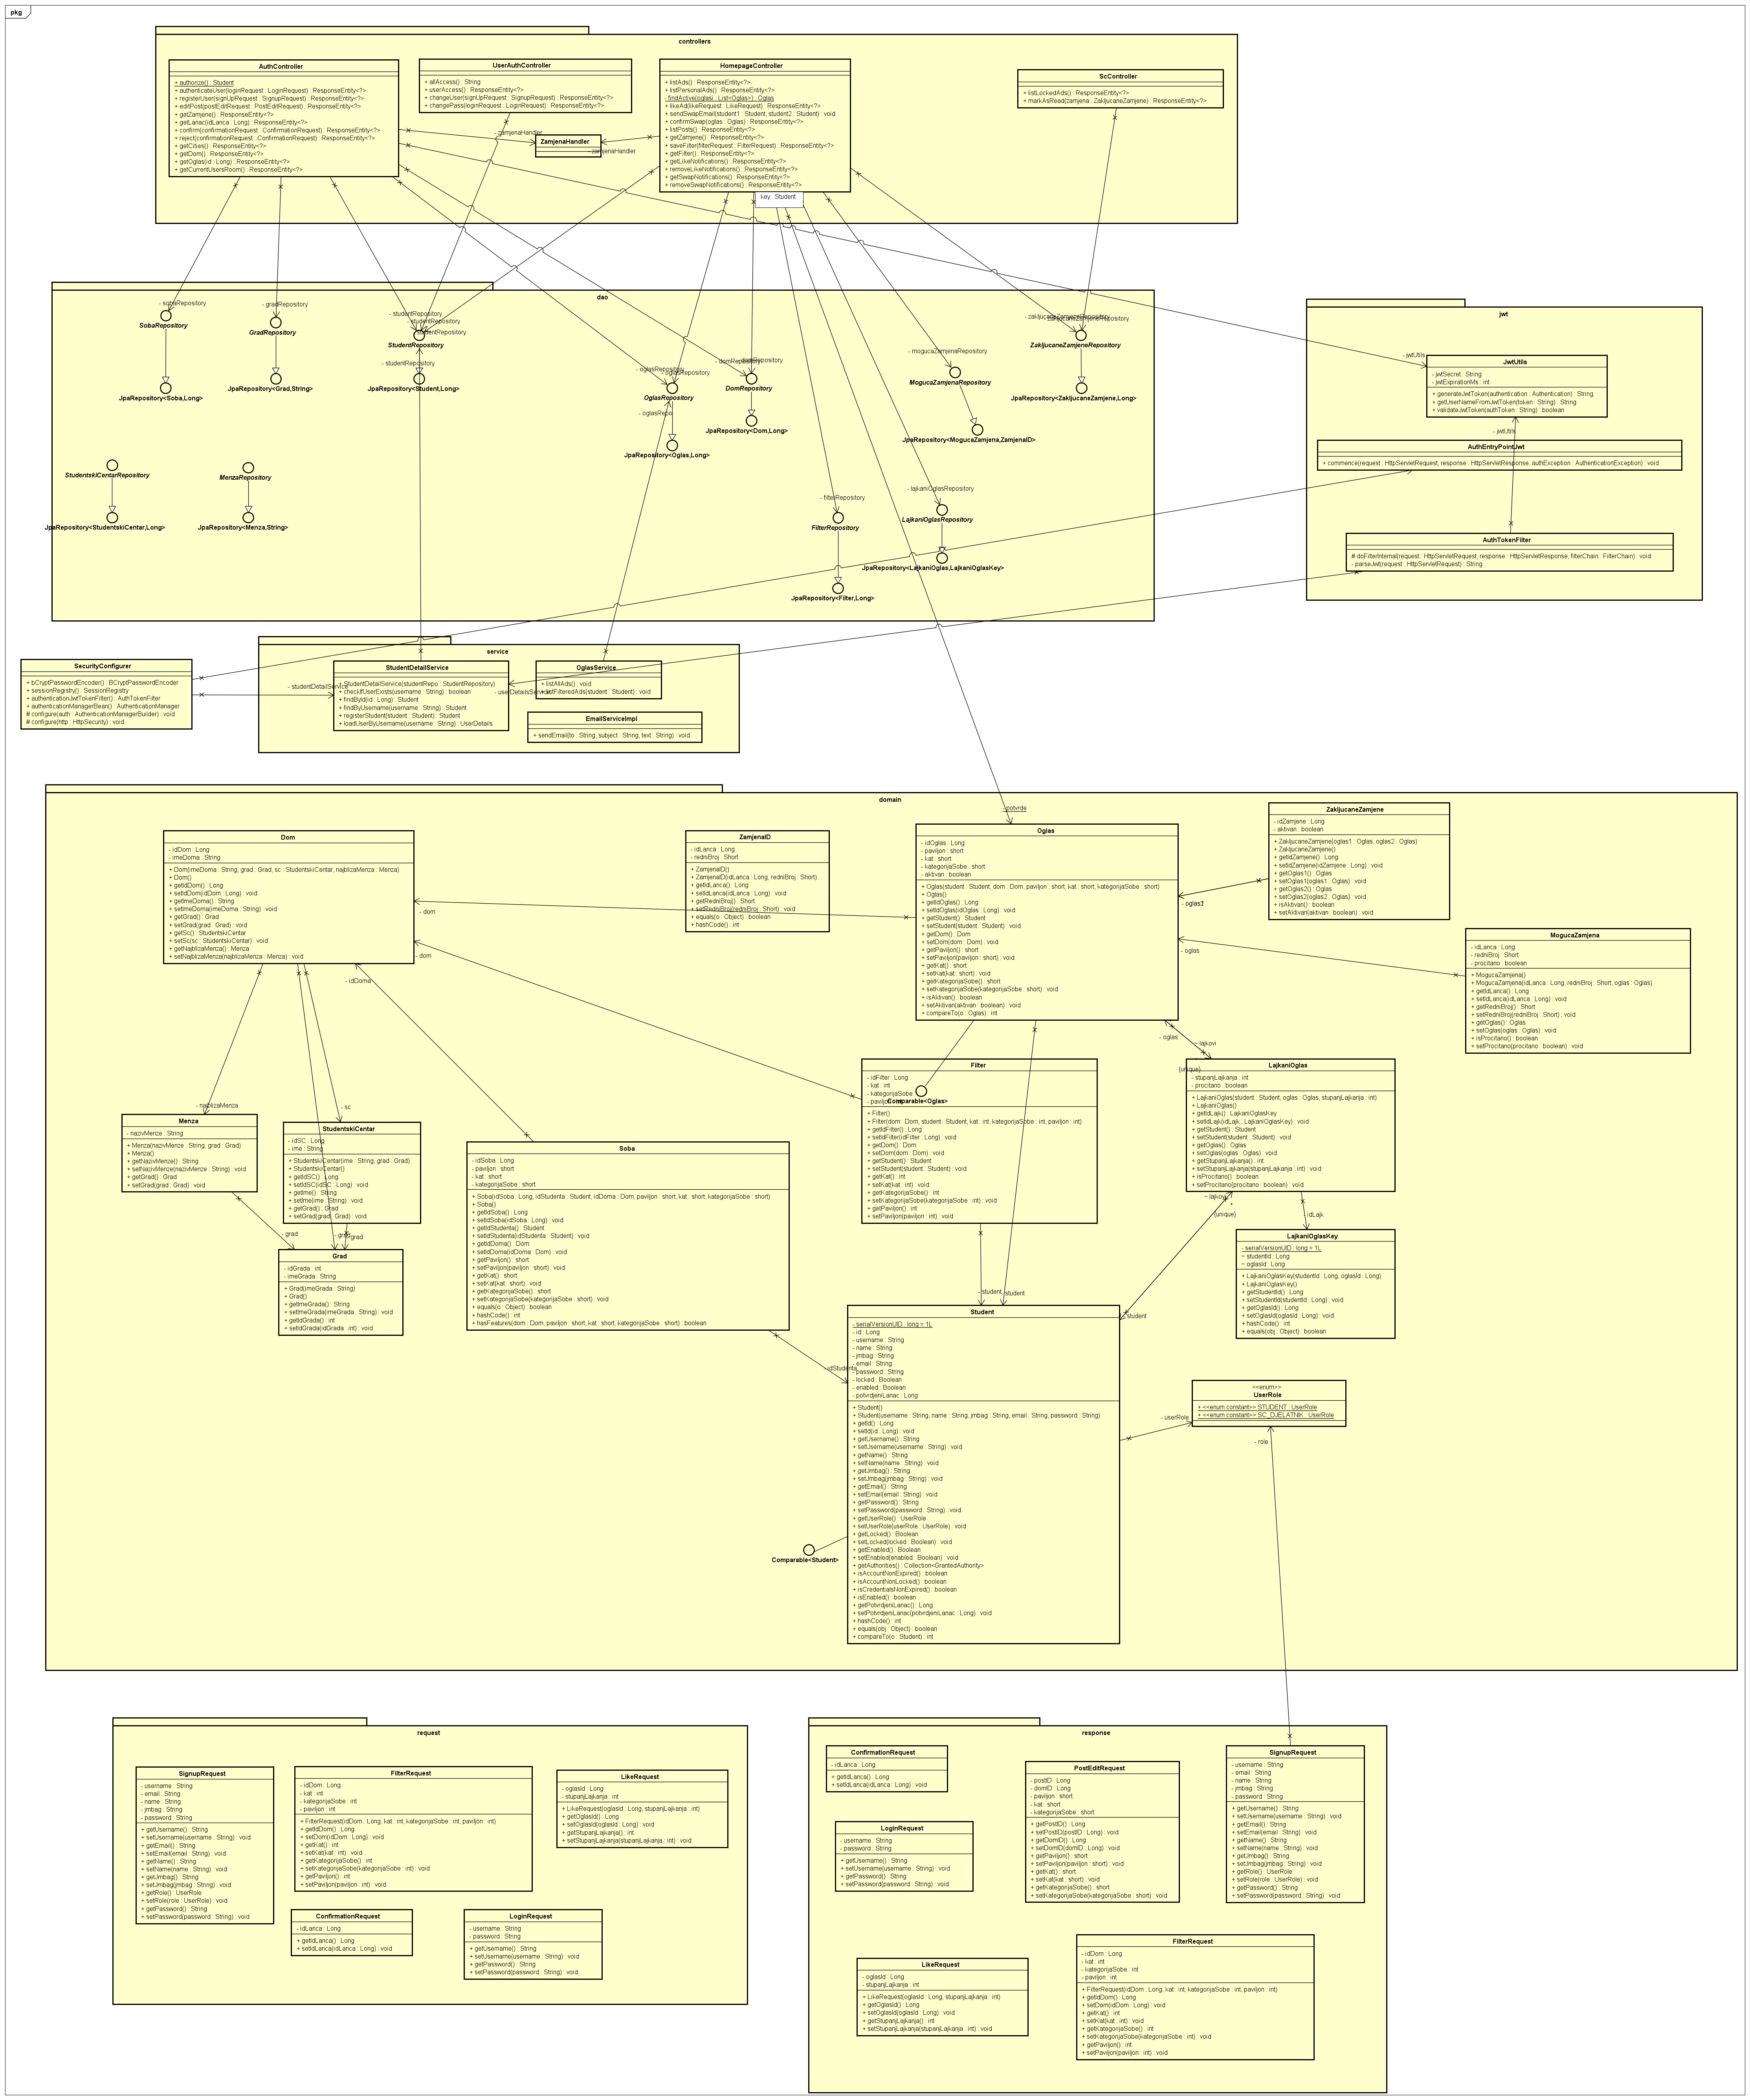
\includegraphics[scale=0.15]{slike/dijag_raz.png} 
			\centering
			\caption{Dijagram razreda}
			\label{fig:models}
		\end{figure}
		
		\eject
			
			\section{Dijagram stanja}
			
				\textbf{\textit{}}\\
			
Dijagram stanja prikazuje stanja objekta te prijelaze iz jednog stanja u drugo te-
meljene na dogadajima. Na slici 4.6 prikazan je dijagram stanja za registriranog
korisnika. Nakon prijave, klijentu se prikazuje pocetna stranica na kojoj može pregledati oglase te poželji filtrirati oglase.
Odabrani oglas korisnik može i lajkati. Korisnik može odabirom različitih opcija i urediti vlastiti profil, pregledati predane oglase, stvoriti novi oglas i urediti predani oglas, pregledati oglase osoba koji su lajkali korisnikov oglas (odabirom opcije "Dobiveni lajkovi"). Ukoliko korisnik odabere opciju "Moguće zamjene", može vidjeti sve oglase koji mu se nude za zaključavanje zamjene te zaključati zamjenu.

			\begin{figure}[H]
				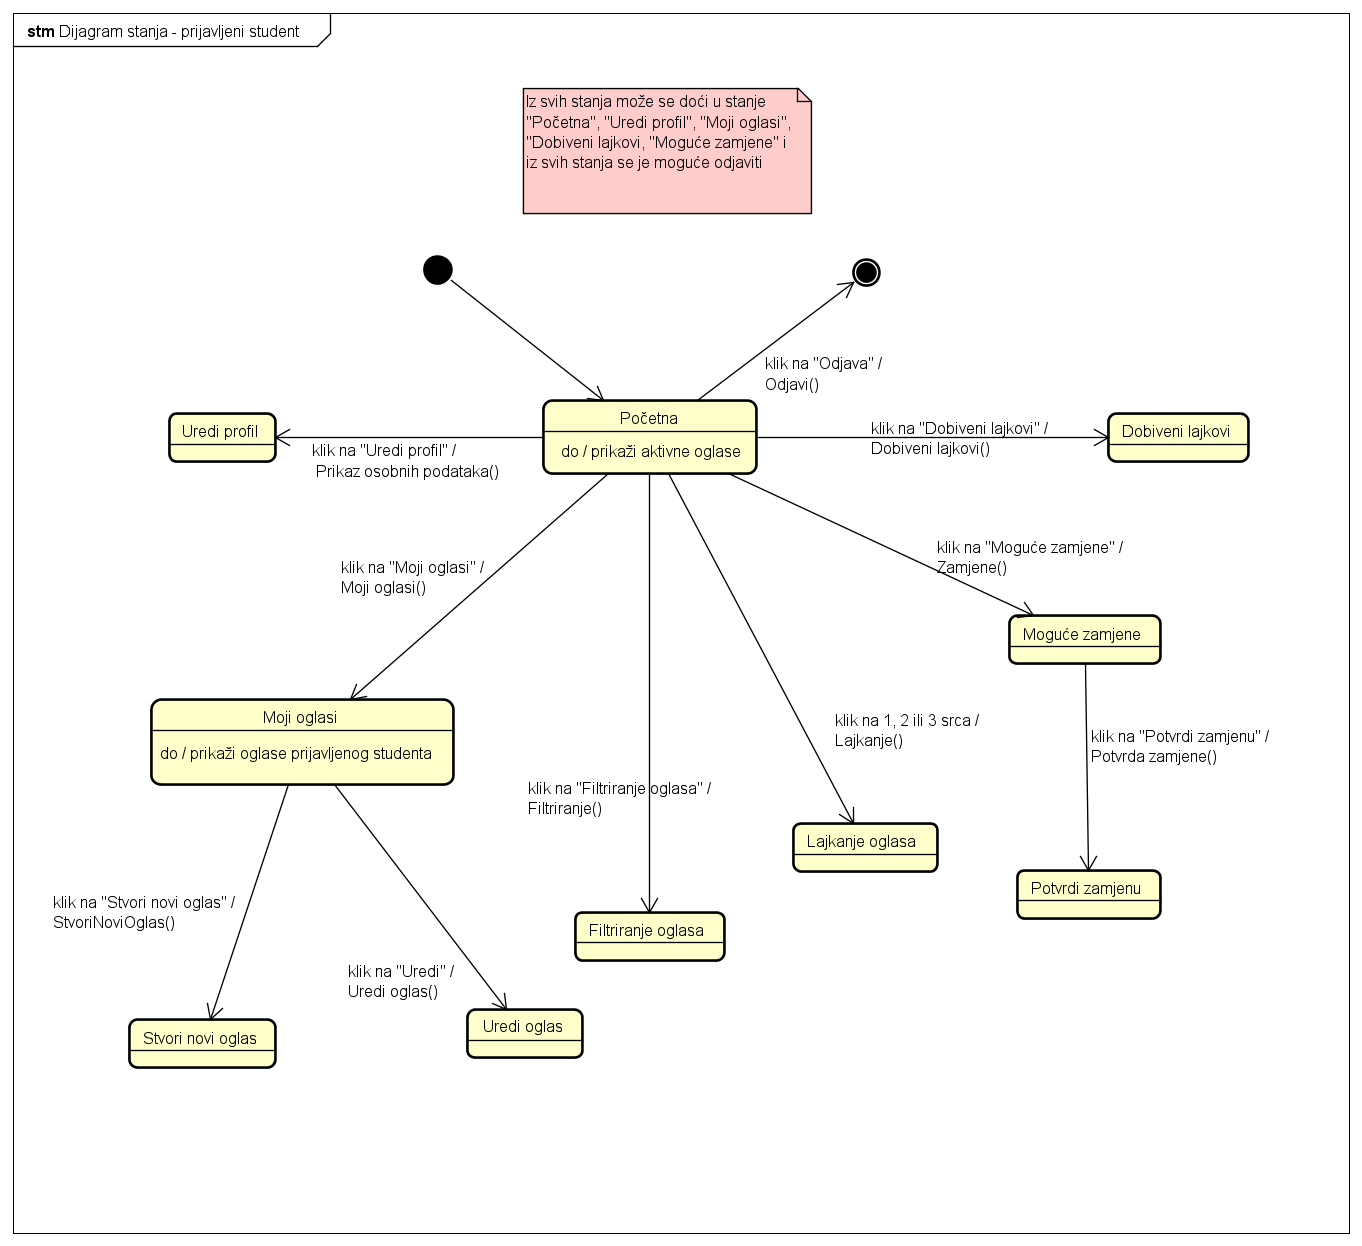
\includegraphics[scale=0.3]{slike/Dijagram_stanja_prijavljeni_student.PNG} %veličina slike u odnosu na originalnu datoteku i pozicija slike
				\centering
				\caption{Dijagram stanja}
				\label{fig:dijagramStanja}
			\end{figure}
			
			
			\eject 
			
			\section{Dijagram aktivnosti}
			
			\textbf{\textit{}}\\
			
			Dijagram aktivnosti primjenjuje se za opis modela toka upravljanja ili toka po-
dataka. Ne upotrebljava se za modeliranje dogadajima poticanog ponasanja. U 
modeliranju toka upravljanja svaki novi korak poduzima se nakon završenog prethodnog, a naglasak je na jednostavnosti. Na dijagramu aktivnosti 4.7 prikazan je
proces lajkanja oglasa. Korisnik nakon prijave u sustav ima uvid u predane oglase. On zatim može odabrati i lajkati neki od prikazanih oglasa ili unijeti filtere za pretraživanje oglasa. Ukoliko korisnik odabere opciju za filtriranje oglasa, sustav će mu prikazati samo one oglase koji odgovaraju njegovim kriterijima te korisnik onda po želji lajka. Nakon što korisnik lajka oglas, promjene se unose u sustav i korisniku se prokazuje uspješno lajkanje u obliku obojanih srca koji su ranije bili bijeli.
			
			\begin{figure}[H]
				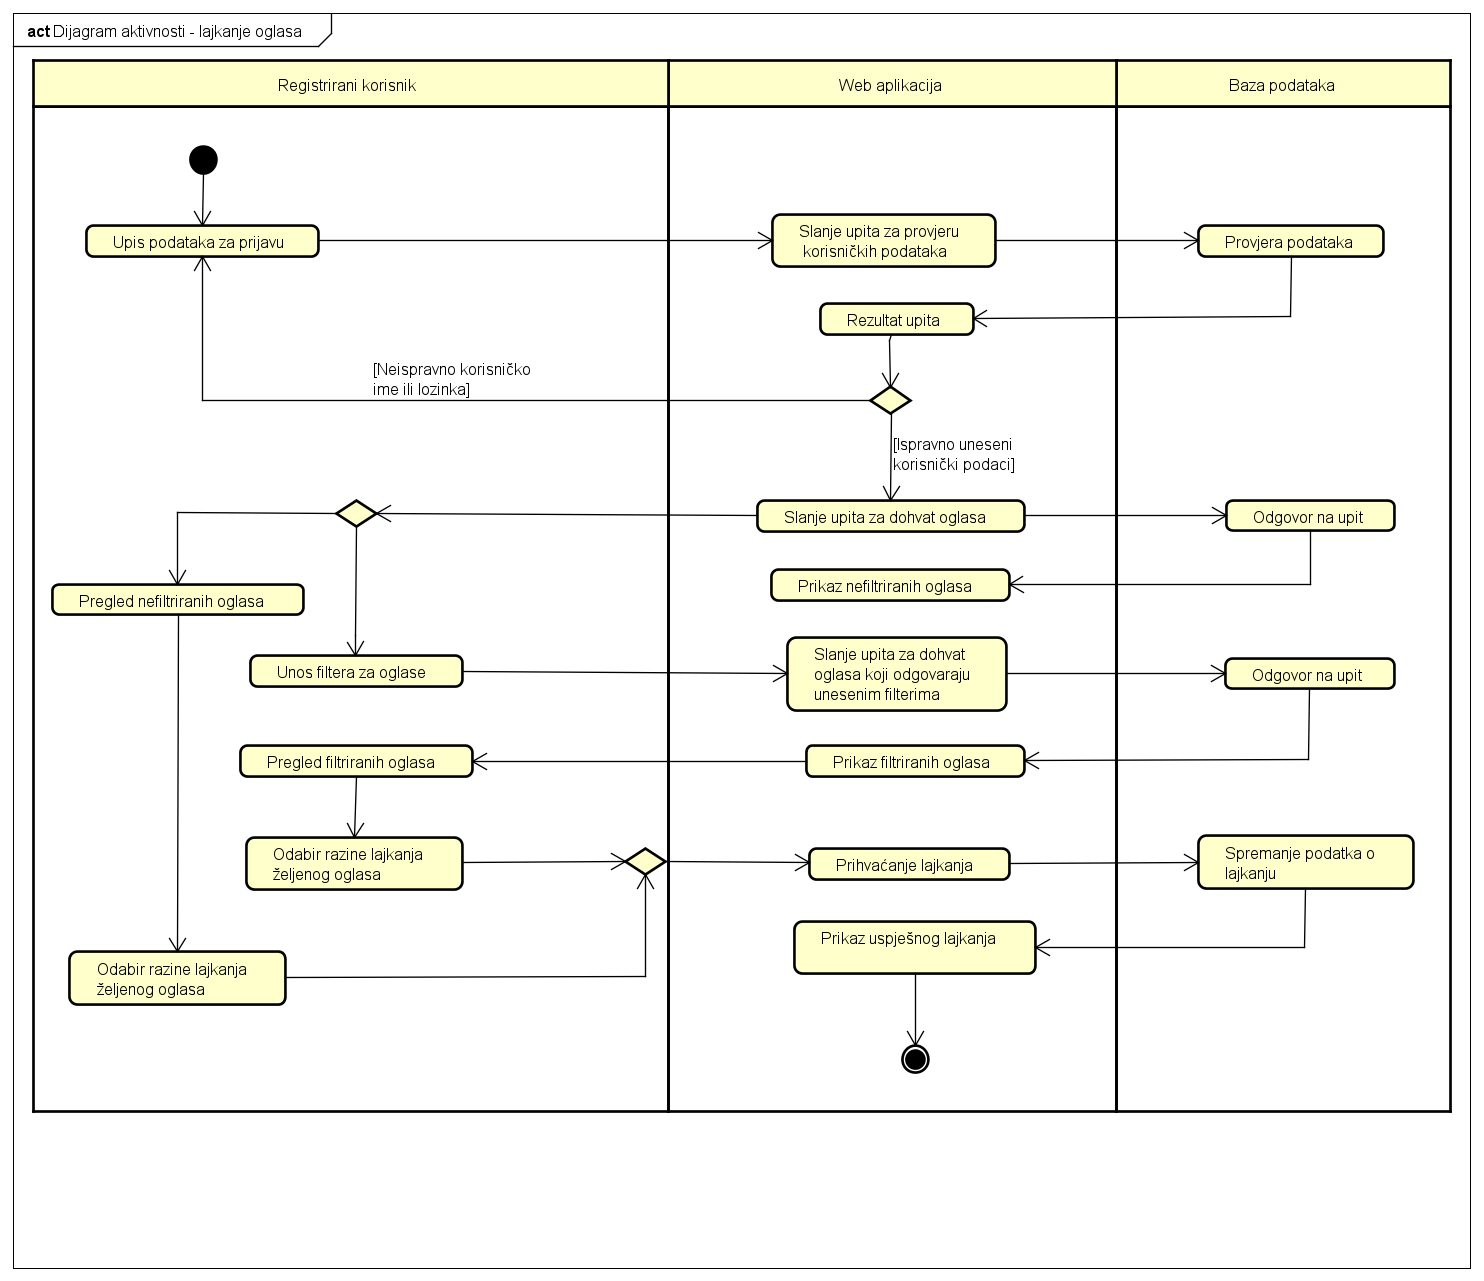
\includegraphics[scale=0.4]{slike/dijagram_ativnosti.PNG} %veličina slike u odnosu na originalnu datoteku i pozicija slike
				\centering
				\caption{Dijagram aktivnosti}
				\label{fig:dijagramAktivnosti}
			\end{figure}
			
			
			\eject
			
			\section{Dijagram komponenti}
			
			Dijagram komponenti prikazan na slici 4.8 opisuje organizaciju i međuovisnost
komponenti, interne strukture i odnose prema okolini. Sustavu se pristupa preko
dva različita sučelja. Preko sučelja za dohvat HTML, CSS i JS datoteka poslužuju se datoteke koje pripadaju frontend dijelu aplikacije. Router je komponenta koja na
upit s url odreduje koja datoteka ce se poslužiti na sučelje. Frontend dio se sastoji
od niza JavaScript datoteka koje su raspoređene u logičke cjeline nazvane po tipovima aktora koji im pristupaju. Sve JavaScript datoteke ovise o React biblioteci iz
koje dohvacaju gotove komponente kao što su gumbi, forme i slično. Preko sučelja za dohvat JSON podataka pristupa se REST API komponenti. REST API poslužuje podatke koji pripadaju backend dijelu aplikacije. EntityFrameworkCore je zadužen za dohvaćanje tablica iz baze podataka pomoću SQL upita. Reactview komponenta preko dostupnih sučelja komunicira s aplikacijom te ovisno o korisnikovim akcijama osvježava prikaz i dohvaća nove podatke ili datoteke.

			
			\begin{figure}[H]
				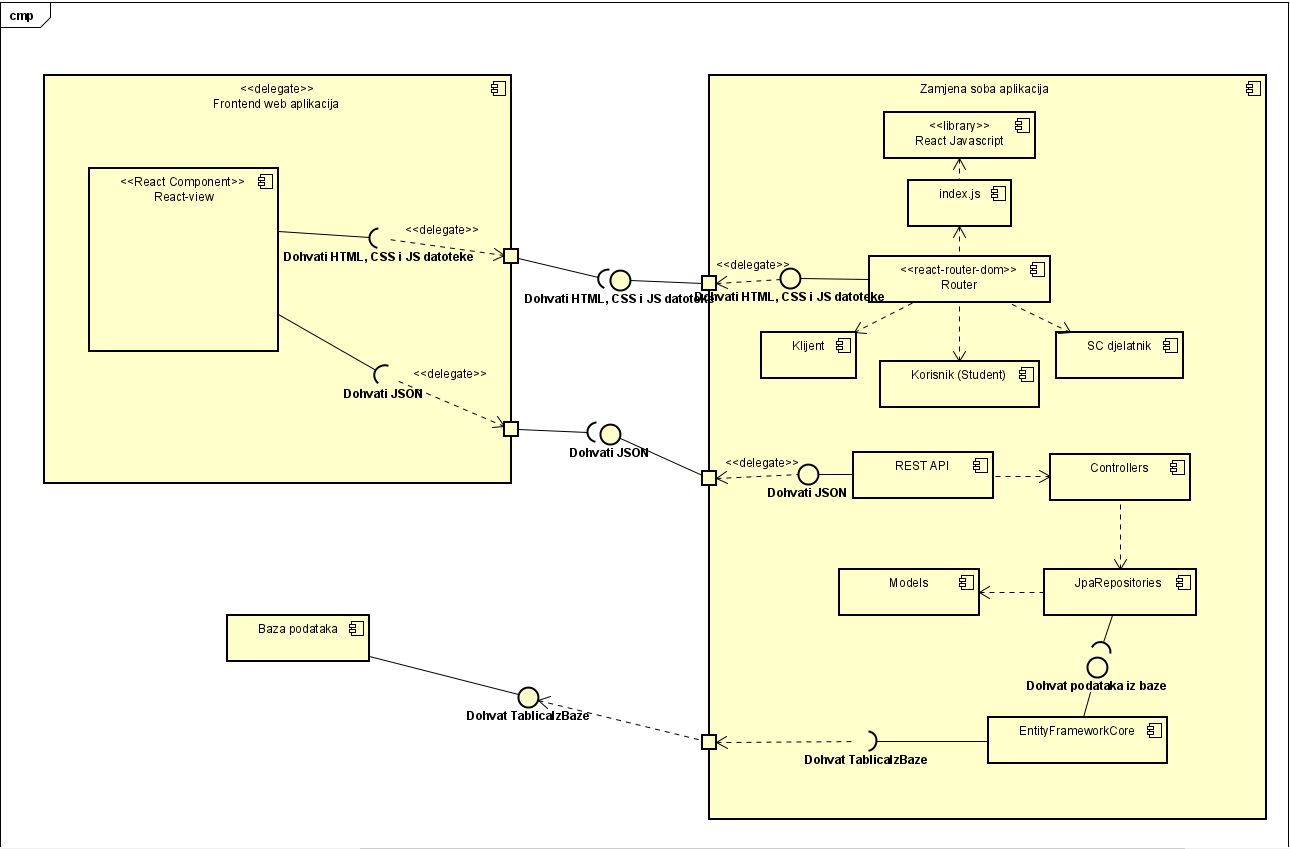
\includegraphics[scale=0.4]{slike/dijagram_komponenti.png} %veličina slike u odnosu na originalnu datoteku i pozicija slike
				\centering
				\caption{Dijagram komponenti}
				\label{fig:dijagramKomponenti}
			\end{figure}
			
			\eject
			
			
			
			